\documentclass{ReportTemplate}
\usepackage{titlesec}
\title{CSEL}
\author{Macherel Rémy}
\date{\today}
\subtitle{Rapports des TP}
\subsubtitle{Git du projet : \href{https://github.com/Mathistis/csel-workspace}{https://github.com/Mathistis/csel-workspace}}
\location{Fribourg,}
\contact{remy.macherel@master.hes-so.ch}
\version{1.0}
\titlespacing*{\chapter}{0pt}{-60pt}{20pt}
\begin{document}

\maketitlepage

\newpage

\maketableofcontent

\medskip

\titleformat{\chapter}[display]
    {\Huge\bfseries}
    {}
    {0pt}
    {\thechapter.\ }
    

\chapter{TP Systèmes de fichiers}

\section{Résumé du travail pratique}
Ce travail consiste à réaliser une application qui contrôle la fréquence de
clignotement d'une LED sur la carte NanoPi. L'application doit permettre grâce
aux systèmes de fichiers et en passant par les boutons de la board de régler la
fréquence de la LED. Un programme de base (silly\_led\_control.c) est fourni
mais celui-ci consomme l'entièreté d'un coeur du processeur. Il nous est donc
demandé de développer un programme qui utilise les systèmes de fichiers pour
contrôler la LED ainsi que les boutons et qui fonctionnerait de manière plus optimisée.

\section{Infos utiles à retenir}
Pour obtenir le numéro de GPIO correspondant à une pin, il faut lire la
configuration à l'aide de la commande :
\begin{minted}[linenos=false]{shell}
mount -t debugfs none /sys/kernel/debug
cat /sys/kernel/debug/gpio
\end{minted}
Afin d'utiliser des event produits par les gpio associés aux boutons, il est
nécessaire d'utiliser \textit{EPOLLERR} car en utilisant \textit{EPOLLIN} cela
ne fonctionne pas. Nous n'avons pas réellement trouvé la raison de ceci et
suspectons un bug dans le kernel. %TODO: Expliquer mieux
Pour les boutons, au moment du open sur le fd, il faut faire un pread pour
quittancer l'interruption alors que pour le timer le read suffit.
\section{Feedback global}
Nous avons dû retrouver dans un ancien TP les numéros de pin des boutons de la
carte car en utilisant les commandes de la section précédente, si ceux-ci ne
sont pas activés cela ne les affiche pas.

\chapter{TP 5 - Ordonnanceur}
\section{Résumé du laboratoire}
Le but de ce laboratoire est de mettre en pratique la théorie vue dans le cours
en ce qui concerne le multiprocessing ainsi que les ordonnanceurs. Il se compose
de deux exercices, un sur les processus et signaux de communication et l'autre
sur l'utilisation des CGroups. Les réponses aux questions ainsi que les
difficultés rencontrées ou information utiles à retenir seront détaillés dans
plus loin dans ce document.

\section{Réponses aux questions}
\subsection{Quel effet a la commande echo \$\$ > ... sur les cgroups ?}
L'utilisation des caractères \textit{\$\$} permet d'obtenir le PID du processus
actuel et donc dans notre cas du shell duquel sera lancé le processus. Cette
commande permet donc de définir les limites de ressources que pourra utiliser
notre processus. Il est utile de préciser que tout processus enfant du shell
(correspondant au PID \$\$) auront les mêmes limites.
\subsection{Quel est le comportement du sous-système memory lorsque le quota de mémoire est épuisé ? Pourrait-on le modifier ? Si oui, comment ?}
See
\href{https://www.kernel.org/doc/Documentation/cgroup-v1/memory.txt}{Doumentation
on cgroups about memory - 2.5 Reclaim}.\newline
Selon la documentation, chaque cgroup maintient une LRU (Least Recently used)
pour sa mémoire. Lorsque la limite est atteinte, il essaie d'abord de récupérer
une mémoire potentiellement disponible mais dans le cas contraire il invoque la
routine OOM (Out Of Memory, voir doc 10. OOM Control). La routine OOM implemente
un notifier utilisant l'api de notifications du cgroup. Il permet d'enregistrer
des notifications de dépassement de mémoire. Le OOM-Killer se charge quant à lui
de stopper les tâches ayant dépassé leur limite en attendant qu'elles en aient à
nouveau.\newline
Lorsque la limite est attente le sous-système ne permet plus d'allocation et
retourne un pointeur vide à chaque essai d'allocation.
\subsection{Est-il possible de surveiller/vérifier l’état actuel de la mémoire ? Si oui, comment ?}
Il est possible de surveiller l'état de la mémoire à l'aide de commandes telles
que \textit{top} ou \textit{htop}. Ces commandes peuvent être utilisées sans
arguments si l'on souhaite surveiller l'état global de la mémoire et des
ressources. Cependant, si l'on veut surveiller un processus en particulier, on
peut utiliser celles-ci de la manière suivante:
\begin{minted}[linenos=false]{shell}
top -p <PID>
\end{minted}
\newpage
Il existe plusieurs outils de ce type pour surveiller l'état de la mémoire et
des ressources. Une liste de certains d'entre eux est disponible
\href{https://geekflare.com/fr/process-cpu-memory-monitoring/}{ici}.
Il est également possible de surveiller ceci en utilisant les fichiers de
\textit{/proc/} qui est ce que l'on appelle un pseudo file system.
(\href{https://man7.org/linux/man-pages/man5/proc.5.html}{doc proc}).
On peut optenir l'espace d'adressage avec la commande :
\begin{minted}[linenos=false]{shell}
cat /proc/<PID>/maps # or smaps
\end{minted}
On peut également obtenir les stats et le status avec les commandes :
\begin{minted}[linenos=false]{shell}
cat /proc/<PID>/status # status
cat /proc/<PID>/statm # stat
\end{minted}
Ces méthodes ne font cependant pas appel aux cgroups. Si l'on souhaite
surveiller nos ressources en utilisant les cgroups à l'aide du \textit{CPU
Accounting Controller}. Il peut être créé de la manière suivante:
\begin{minted}[linenos=false]{shell}
mount -t cgroup -ocpuacct none /sys/fs/cgroup
cd /sys/fs/cgroup
mkdir g1 #group name can be changed 
echo $$ > g1/tasks #add current process to group
\end{minted}
On peut utiliser \textit{/sys/fs/cgroup/g1/cpuacct.usage} pour obtenir les temps
CPU (en nanosecondes) obtenus par ce groupe.
\textit{/sys/fs/cgroup/g1/cpuacct.stat} liste quelques statistiques comme par
exemple:
\begin{itemize}
    \item user : le temps passé par les tâches du cgroup en user mode.
    \item system : Le temps passé par les tâches du cgroup en mode kernel.
\end{itemize}
Plus d'informations sur ce type de cgroup sont disponibles
\href{https://www.kernel.org/doc/html/latest/admin-guide/cgroup-v1/cpuacct.html}{ici}.
\newline
Il existe aussi des memory controllers comme ceux utilisés pour la limitation de
mémoire. Il existe des moyens de controller l'usage de mémoire avec le cgroup
memory.usage\_in\_bytes. Des possibilités comme memory.failcnt ou stat
permettent d'obtenir des informations comme le nombre de fois que la limite de
mémoire a été atteinte ou d'afficher diverses statistiques.
(\href{https://www.kernel.org/doc/html/latest/admin-guide/cgroup-v1/memory.html}{cgroup
memory}).
\subsection{Les 4 dernières lignes sont obligatoires pour que les prochaines commandes fonctionnent correctement. Pouvez-vous en donner la raison ?}
Les lignes 1 et 3 servent à définir le cpu sur lequel chacun des cgroups pourra
exécuter ses tâches. Les deux autres écrivant 0 dans cpuset.mems servent à
définir le noeud mémoire que va utiliser le cgroup. Ceci est souvent utilisé sur
les systèmes à architecture NUMA (Non Uniform Memory Access) signifiant que le
système peut contenir plusieurs types de mémoires différents symbolisés par des
noeuds. Dans le cas du Nanopi nous n'avons qu'une seule mémoire et donc la
documentation préconise d'inscrire 0 dans cpuset.mems pour les systèmes n'ayant
pas de NUMA. (Info trouvée \href{https://docs.oracle.com/cd/E37670_01/E37355/html/ol_cpuset_cgroups.html#:~:text=mems%20changes.,the%20node%20list%20where%20possible.}{ici}). 
\newpage
\subsection{Comportement des shells dans deux cgroups différents}
On observe que chaque application utilise le 100\% du coeur qui lui est affecté.
Les deux processus à l'intérieur de chaque application doivent par conséquent se
partager le coeur pour leur exécution. On peut observer ceci sur la figure
suivante:
\begin{figure}[H]
    \centering
    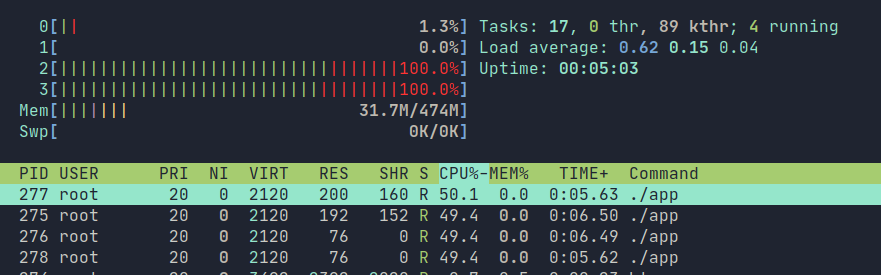
\includegraphics[width=0.7\textwidth]{imageSources/LowHigh_Groups.png}
    \caption{Two different shells executing app}
    \label{fig:LowHighGroup}
\end{figure}
On observe ici que la barre d'utilisation des coeurs 2 et 3 est à 100\% mais
avec deux couleurs ce qui représente les deux processus de chaque application se
partageant le coeur.
\subsection{Sachant que l’attribut cpu.shares permet de répartir le temps CPU entre différents cgroups, comment devrait-on procéder pour lancer deux tâches distinctes sur le cœur 4 de notre processeur et attribuer 75\% du temps CPU à la première tâche et 25\% à la deuxième ?}
Nous avons procédé de la manière suivante : \newline
Nous avons gardé les deux cgroup de la question précédente (Low et High) mais
cette fois affecté le coeur 4 aux deux tâches. Nous avons ensuite défini à
l'aide de l'attribut cpu.shares que le premier groupe (High) peut occuper 75\% du temps
du coeur et le deuxième (Low) uniquement 25\%.
Pour ce faire nous avons trouvé dans la documentation que la valeur 1024 dans
cpu.shares correspondait au 100\% du coeur nous avons donc mis 768 dans cet
attribut pour le High cgroup et 256 pour le Low. On peut voir sur la figure
suivante que le coeur 4 est occupé à 100\% par 4 processus (deux pour chaque
tâche), et que pour la tâche appartenant au groupe 1, les processus utilisent
environ 37.5\% chacun alors que pour la tâche appartenant au groupe 2, les
processus utilisent environ 12.5\% de du coeur. Ainsi on peut voir que la tâche
1 (appartenant au groupe High) utilise bien 75\% du coeur et la tâche 2
(appartenant au groupe Low) utilise bien 25\%.
\begin{figure}[H]
    \centering
    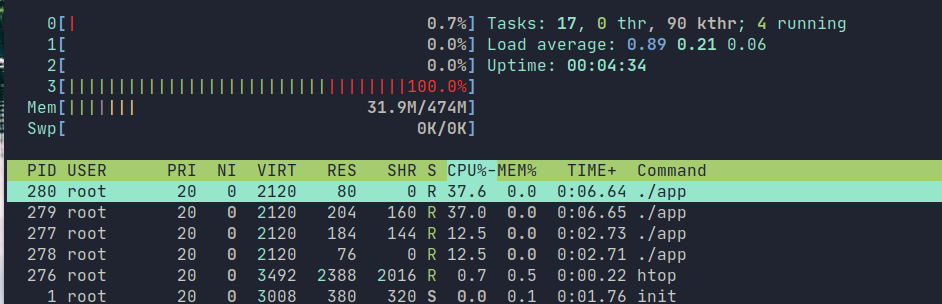
\includegraphics[width=0.7\textwidth]{imageSources/75x25Use.png}
    \caption{75\% and 25\% of the CPU on core 4}
    \label{fig:LowHighGroup2}
\end{figure}
\newpage
\section{Synthèse des connaissances acquises}
\subsection{Non acquis}
Nous n'avons pas réellement décelé des connaissances que nous pourrions
qualifier de non-acquises. En effet, après avoir suivi le cours et réalisé les
TP, cela nous a permis de comprendre la matière ciblée par ce travail pratique.
\subsection{Acquis, mais à exercer}
Le domaine d'utilisation des cgroups afin de limiter les ressources disponibles pour des
processus est très vaste et ce travail pratique nous a permis d'en découvrir
quelques facettes mais nous pensons que ce sont des aspects que nous pourrions
mieux aprofondir avec plus de pratique.
\subsection{Parfaitement acquis}
Comme cité précedemment dans la section des connaissances à exercer, nous ne
pourrions pas dire que nous avons parfaitement acquis les connaissances
relatives aux cgroups, mais nous les avons cependant bien comprises et nous
sommes en mesure de pouvoir affirmer que nous saurions les réutiliser.
\section{Infos utiles à retenir}
La fonction c \textit{strcmp} retourne la valeur 0 quand les deux chaînes de
caractères sont identiques. Nous nous sommes faits avoir par ceci et avons perdu
passablement de temps à chercher une erreur alors qu'elle se trouvait simplement
à cet endroit.\newline
Lors de la capture des signaux, si l'on capture un signal alors que le processus
était en \textit{sleep}, à la fin du traitement de la capture le signal sera
réveillé car en effet cela reprend l'exécution du processus là ou il en était
mais dans le cas d'un sleep ne vérifie pas que celui-ci soit terminé. Si l'on
voulait s'assurer que le temps du sleep soit bien respecté il faudrait utiliser
le fait que la fonction sleep lorsqu'elle est interrompue retourne le nombre de
secondes restantes à son exécution. On pourrait donc comparer à la suite de
l'instruction sleep si le temps restant est de 0 ou non et dans le cas contraire
replonger le processus en sommeil pour la durée de temps restante. De plus, dans
le cas d'un besoin de précision il est conseillé d'utiliser \textit{clock\_nanosleep} au lieu de \textit{sleep}.
\newpage
\section{Feedback exercices}
\subsection{Exercice 1}
Nous avons réalisé cet exercice en utilisant un \textit{socketpair} afin de
communiquer entre deux processus. Le processus parent envoie via le socket des
messages au processus enfant qui les affiche dans la console. Le processus
enfant "répond" en affichant simplement dans la console car nous n'avons pas eu
le temps de développer le fait qu'il renvoie un message dans le socketpair. Une
fois le message correspondant à l'ordre de quitter reçu, le processus enfant se
termine. Dans le main, le processus parent attend grace à la fonction
\textit{wait} la fin du processus enfant.\newline
L'étape suivante consistait à capturer et ignorer tous les signaux (sauf le 9
SIGSTOP et le 19 SIGKILL) et juste afficher un message à la réception d'un
signal. Nous avons suivi la procédure du cours ainsi que quelques recherches et
donc parcouru une boucle de 30 (correspondant aux 30 signaux p. 8 du cours) afin
de tous leur affecter une \textit{sigaction} permettant de les ignorer.\newline
La dernière partie consistait à dispatcher les deux processus sur deux coeurs
différents du nanopi. Pour ce faire nous avons utilisé les fonctions suivantes :
\begin{minted}[linenos=false]{c}
    cpu_set_t set;
    CPU_ZERO(&set);
    CPU_SET(1, &set); // set to the core 1
    int ret = sched_setaffinity(0, sizeof(set), &set);
\end{minted}
Et ceci pour les deux processus. Notre application étant très rapidement
exécutée et afin de vérifier le bon fonctionnement de ceci, nous avons ajouté
dans le code une boucle \textit{while} d'un grand nombre d'itérations effectuant
une multiplication et un print afin de visualiser à l'aide de \textit{htop}
l'utilisation des coeurs comme le montre la figure suivante :
\begin{figure}[H]
    \centering
    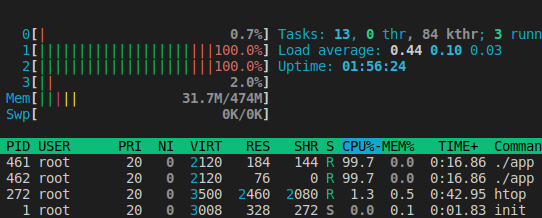
\includegraphics[width=0.7\textwidth]{imageSources/MultiCPU.png.png}
    \caption{Multi Core usage}
    \label{fig:MultiCore}
\end{figure}

\subsection{Exercice 2}
Il a été observé que si l'on lance le programme et que l'on essaie de limiter le
nombre de bytes possibles alors qu'il a déjà atteint le quota, l'écriture est
bloquée et la limite ne peut être fixée. Cependant si l'on écrit la limite avant
que le programme ne l'ait atteinte, elle sera bien fixée et le programme
s'arrêtera lorsqu'il atteindra cette limite.\newline
Commande pour limiter la quantité max de mémoire :
\begin{minted}[linenos=false]{shell}
echo 20M > /sys/fs/cgroup/set/program/memory.limit_in_bytes
\end{minted}

Nous avons également pu observer que si l'on crée deux cgroup de limitation de
mémoire, un de 20M et l'autre de 30M. Si l'on ajoute notre PID dans celui de 20M
puis dans celui de 30M, au moment de l'ajout dans celui de 30M il est
automatiquement retiré des tasks du cgroup qui limitait à 20M.\newline

Nous avons créé un script pour limiter la mémoire et celui-ci se lance de la
manière suivante : 
\begin{minted}[linenos=false]{shell}
    ./set_memory_limit <PID> <MEMORY_LIMIT>
\end{minted}
\subsection{Exercice 3}
Nous avons également pu observer que si l'on crée deux cgroup de limitation de
mémoire, un de 20M et l'autre de 30M. Si l'on ajoute notre PID dans celui de 20M
puis dans celui de 30M, au moment de l'ajout dans celui de 30M il est
automatiquement retiré des tasks du cgroup qui limitait à 20M.

\chapter{TP 6 - Optimisation}
\section{Résumé du laboratoire}
Ce laboratoire permet de prendre en main l'outil \href{https://man7.org/linux/man-pages/man1/perf.1.html}{\textit{perf}} et de tester
quelques unes de ses fonctionnalités. Nous avons préalablement installé cet
outil dans le buildroot avec les \textit{binutils} associées puis recompilé
celui-ci.
\section{Réponses aux questions}
\subsection{Exercice 1 - Ce programme contient une erreur triviale qui empêche
une utilisation optimale du cache. De quelle erreur s’agit-il ?}

\subsection{Exercice 1 - Relevez les valeurs du compteur L1-dcache-load-misses
pour les deux versions de l’application. Quel facteur constatez-vous entre les
deux valeurs ?}

\subsection{Mesure de l'impact de perf sur la performance du programme}

\section{Synthèse des exercices}
\subsection{Exercice 1}
Afin de corriger le bug nous avons ...
\section{Synthèse des connaissances acquises}
\subsection{Non acquis}

\subsection{Acquis, mais à exercer}

\subsection{Parfaitement acquis}

\section{Feedback}

\end{document}


